\documentclass[border=4pt]{standalone}
\usepackage{fontspec}
\usepackage{amsmath}
\usepackage{unicode-math}
\setmainfont{Latin Modern Roman}
\setmathfont{Latin Modern Math}
\usepackage{pgfplots}
\usepackage{pgfplotstable}
\pgfplotsset{compat=1.18}
\usepackage{tkz-euclide}
\usetikzlibrary{arrows.meta,calc,angles,quotes,patterns,3d,backgrounds}
\definecolor{ink}{HTML}{123428}
\definecolor{asy}{HTML}{475569}
\definecolor{mint}{HTML}{86e0bd}
\tikzset{asym/.style={asy, line width=0.9pt, dash pattern=on 5pt off 3.5pt},
         guide/.style={gray!70, line width=0.6pt, densely dotted},
         dot/.style={circle, inner sep=0pt, minimum size=5pt, draw=white, line width=0.5pt},
         odot/.style={circle, inner sep=0pt, minimum size=5.5pt, fill=white, line width=1pt},
         lab/.style={font=\footnotesize, inner sep=1.5pt, text=ink}}
\begin{document}
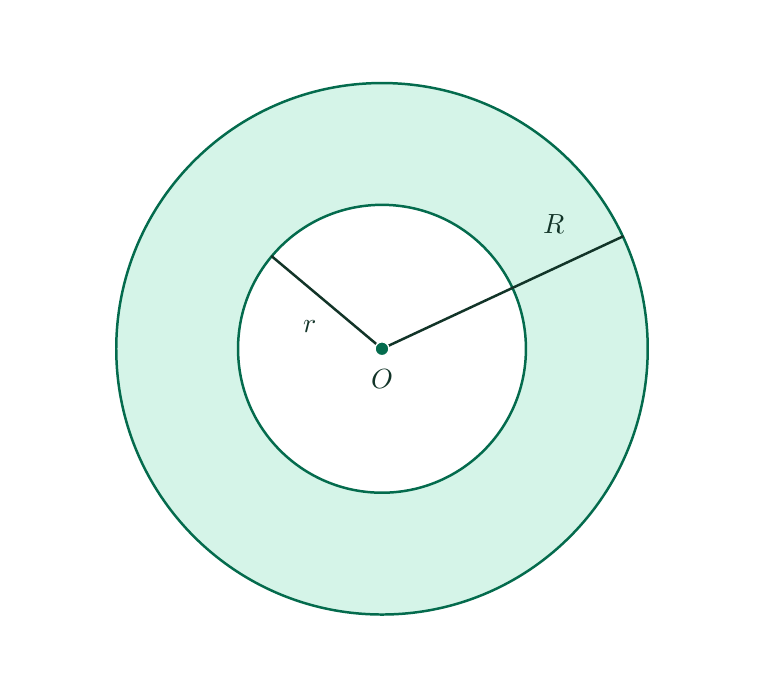
\begin{tikzpicture}[x=1.4062cm, y=1.4062cm]
\tkzDefPoint(0,0){O}
\tkzDefPoint(2.1751,1.0143){P}
\tkzDefPoint(-0.9959,0.8356){Q}
\tkzDefPoint(2.4,0){tmp1}
\tkzDefPoint(1.3,0){tmp2}
\begin{scope}
\clip (-3.2,-2.9) rectangle (3.2,2.9);
\tkzDrawCircle[draw={rgb,255:red,4;green,107;blue,77}, line width=0.9pt, fill=mint, fill opacity=0.35](O,tmp1)
\tkzDrawCircle[draw={rgb,255:red,4;green,107;blue,77}, line width=0.9pt, fill={rgb,255:red,255;green,255;blue,255}, fill opacity=1](O,tmp2)
\tkzDrawSegment[draw=ink, line width=0.90pt](O,P)
\tkzDrawSegment[draw=ink, line width=0.90pt](O,Q)
\end{scope}
\node[dot, fill={rgb,255:red,4;green,107;blue,77}] at (O) {};
\node[lab, font=\normalsize] at (1.55,1.12) {$R$};
\node[lab, font=\normalsize] at (-0.65,0.2) {$r$};
\node[lab, font=\normalsize, anchor=center, xshift=0pt, yshift=-11pt] at (0,0) {$O$};
\end{tikzpicture}
\end{document}
